\subsection{Box Cut and Support Relocation }\label{sec:mirrorRepos}

In the CLAS12 design upgrade the space between the Drift Chambers and the Forward Time-Of-Flight system
was reduced from 2~m to 1.5~m.
In order to accommodate the LTCC in the new space, the original aluminum frame was modified with a cut, see \F{boxCut}.
The mounting structure of the three mirror sets involved in the cut was repositioned. For this work, new threaded holes were
drilled in the frame and the old holes were plugged and sealed.

\begin{figure}
	\centering
	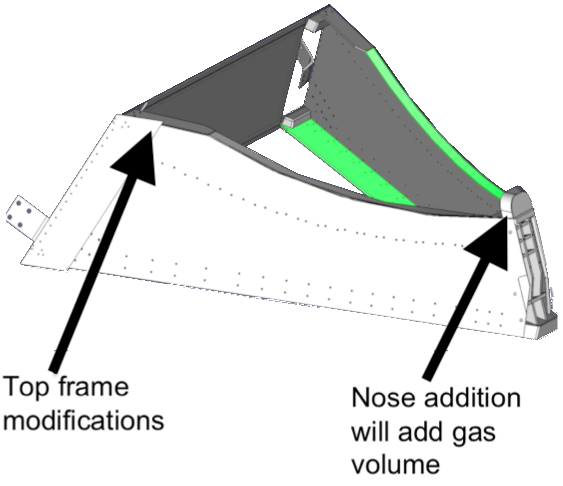
\includegraphics[width=1.0\columnwidth, height=0.75\columnwidth]{img/boxCut.png}
	\caption{The refurbished LTCC box frame. Originally the frame walls spanned a portion of the surface of a 5~m
          radius sphere centered on the target. The side-walls had to be cut near the top part of the frame and the four
          mirror sets involved had to be relocated. A stainless steel nose window support was added to the original detector
          to increase the gas volume.}
	\label{fig:boxCut}
\end{figure}

\subsection{Nose Addition and Window Inflation}

In the original design the upstream window followed the spherical curvature of the frame sidewalls. In the new system, the window is
designed to inflate to enlarge the gas volume in order to increase the number of Cherenkov photons. In addition, a ``nose''
support (see \F{boxCut}) has been engineered to increase the gas volume.
The nose dimensions have been optimized to provide the necessary support, while at the same time, maximizing the gas volume increase.
The gas volume increase of the final configuration is shown in \F{noseVolume}.

\begin{figure}
	\centering
	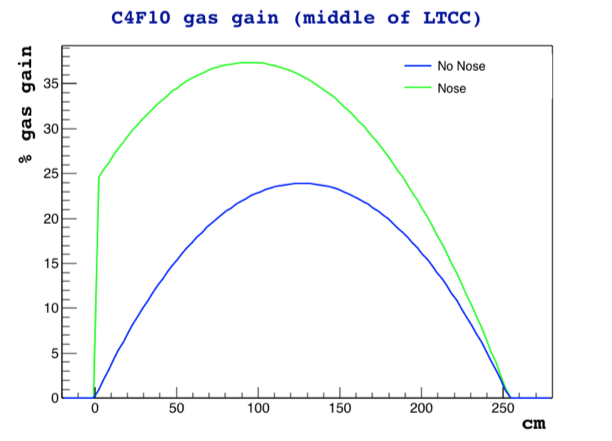
\includegraphics[width=0.98\columnwidth, height=0.7\columnwidth]{img/noseVolume.png}
	\caption{The gas volume percentage gains with and without the nose addition compared to the old CLAS configuration as a function of
            distance from the nose in cm. Dashed: the percentage increase due to the window inflation compared to the original flat design.
            Solid: the additional percentage increase due to the nose addition.}
	\label{fig:noseVolume}
\end{figure}

\subsection{Back-wall and Connectors}

Both the high voltage and the signal connectors that link the PMTs inside the LTCC box and the outside electronics were not
hermetic during CLAS operations and epoxy was used to minimize the leaks from these connectors.
As part of the back-wall refurbishment, the patch panel was rebuilt and hermetic connectors were used.

The new back-wall design is shown in \F{backWall}. The wall is supported by stainless steel bars that enclose a panel made of foam enclosed by
thin aluminum sheets to minimize the radiation length.
The new patch panels provide 3 connectors for each PMT: one for high voltage and two for an identical signal coming from the modified PMT base.
One signal is digitized through a flash ADC and the other one through a discriminator and TDC.

\begin{figure}
	\centering
	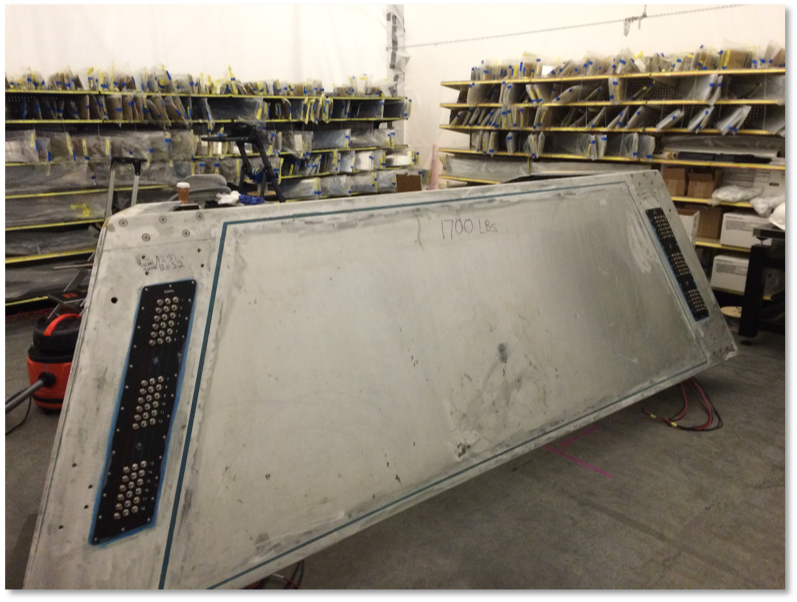
\includegraphics[width=0.99\columnwidth,keepaspectratio]{img/backWall.png}
	\caption{View of the back-wall of the refurbished LTCC box. A stainless steel bar encapsulates a sandwich
             of aluminum and foam. On the left and right side of the frame, new patch panels allow for 3 hermetic
             BNC connectors (1 HV, 2 signals) from each PMT. }
	\label{fig:backWall}
\end{figure}

\subsection{Mirror Support Spine}

When the LTCC boxes were opened for refurbishment, the mirror support spine of all six LTCC sectors was found to be broken.
The spine was an aluminum honeycomb designed to prevent the mirrors from breaking under their own weight.
It was attached to the box nose and the back-wall. The spine was rigid and broke due to small
(of the order of 0.5~cm) deformations of the box when it was transported and/or installed.
A new carbon fiber spine, see \F{spine}, was designed that is capable of floating up to 1 cm, effectively compensating
for the non-rigid movements of the box.
The mirrors are linked to the spine through stainless steel cables 0.127-mm thick.
The cables are anchored with stainless steel springs with tension varying from 0.5 to 1~kg.
The spine was tested by mounting a laser on the box. The laser line was focused through the elliptical
and hyperbolic mirrors to a target in the middle of the covered face of a PMT.
In order to verify that the detector transportation and/or installation would not break the spine
or affect the mirror alignment, the box was lifted, rotated back and forth by 90\mdeg, and subjected
to small vibrations. The focused spot on the PMT did not change with any of these movements and
the spine
compensated for the box wall deformations.

\begin{figure}
	\centering
	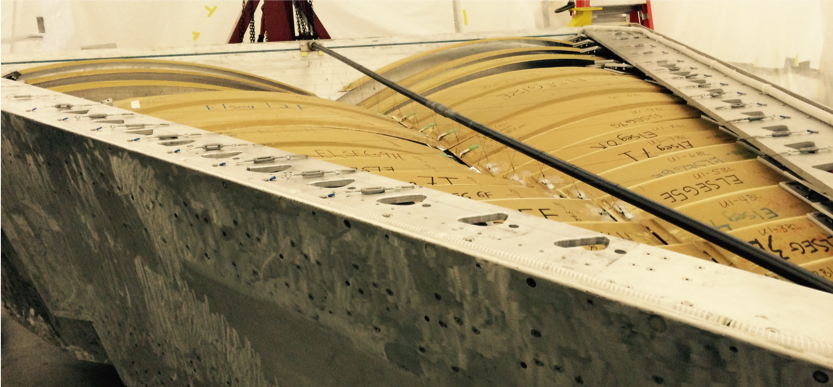
\includegraphics[width=1.0\columnwidth,keepaspectratio]{img/spine.png}
	\caption{The LTCC mirror support spine. The carbon fiber tube (in black) is allowed to float up to 1~cm to compensate
             for possible box deformation during the detector transportation and installation. The mirrors are linked to
             the spine through stainless steel cables 0.127-mm thick and tensioned through springs.}
	\label{fig:spine}
\end{figure}

%\begin{figure}
%	\centering
%	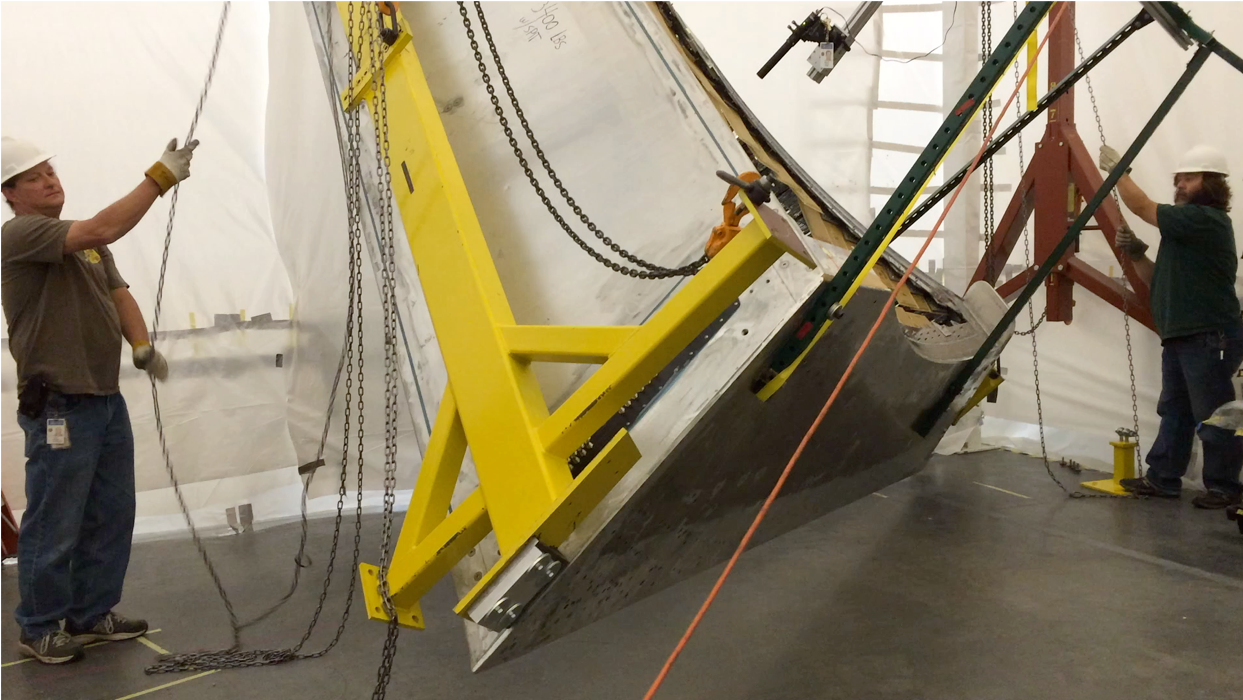
\includegraphics[width=1.0\columnwidth,keepaspectratio]{img/spineTest.png}
%	\caption{Spine tests: a laser was mounted on a structure attached to one LTCC sector, pointing a laser line that was focused by the mirrors to a
%            target on the face of one PMT. The focused laser spot never changed during the box movements and rotations.}
%	\label{fig:spineTest}
%\end{figure}





